% ============================================================
\section{Experiments}
\label{sec:experiments}
% ============================================================

We validate the Ordinal MDP framework through three main experiments: transfer gap decomposition on tabular MDPs, baseline comparisons, and neural policies (DQN on Gymnasium and SAC on MuJoCo). Additional experiments---ordinal stability radius, LQR quadratic degradation (\S\ref{sec:exp-lqr}), control-environment transfer (Wind Grid + Pendulum), sample complexity, and a 4-joint robot surrogate---are deferred to Appendix~\ref{app:additional-exp} for space; multi-dimensional ($d=3$) parameter transfer is in Appendix~\ref{app:exp-multidim}. Code is available in the supplementary material.

% ────────────────────────────────────────────────────────────
\subsection{Transfer Gap Decomposition (Theorem~\ref{thm:transfer-gap})}
\label{sec:exp-transfer-gap}
% ────────────────────────────────────────────────────────────

\paragraph{Setup.} $5 \times 5$ grid-world MDP family parameterized by $\theta \in [0,1]$ controlling wind strength and step cost. Source policy $\pi^*_{\theta_0}$ at $\theta_0 = 0$, deployed across 50 target parameters.

\paragraph{Results.} Our decomposition matches the true gap exactly while the Simulation Lemma overestimates by $3{,}600$--$123{,}700\times$ (Figure~\ref{fig:transfer-gap}(a,b))---it sums over all $|\cS|{=}25$ states (vs.\ $|\Sviol|{\leq}2$), uses worst-case $\Vmax$, and ignores visitation; when $\Sviol{=}\emptyset$ our bound is zero while the Simulation Lemma exceeds $200$. Figure~\ref{fig:transfer-gap}(d) validates Theorem~\ref{thm:violation-growth}: $F_\kappa(2L_Q\|\Delta\theta\|)$ upper-bounds the actual violation fraction at all parameters. Appendix~\ref{app:perstate} confirms the mechanism: states violate in order of increasing $\kappa(s)$.

\begin{figure}[t]
\centering
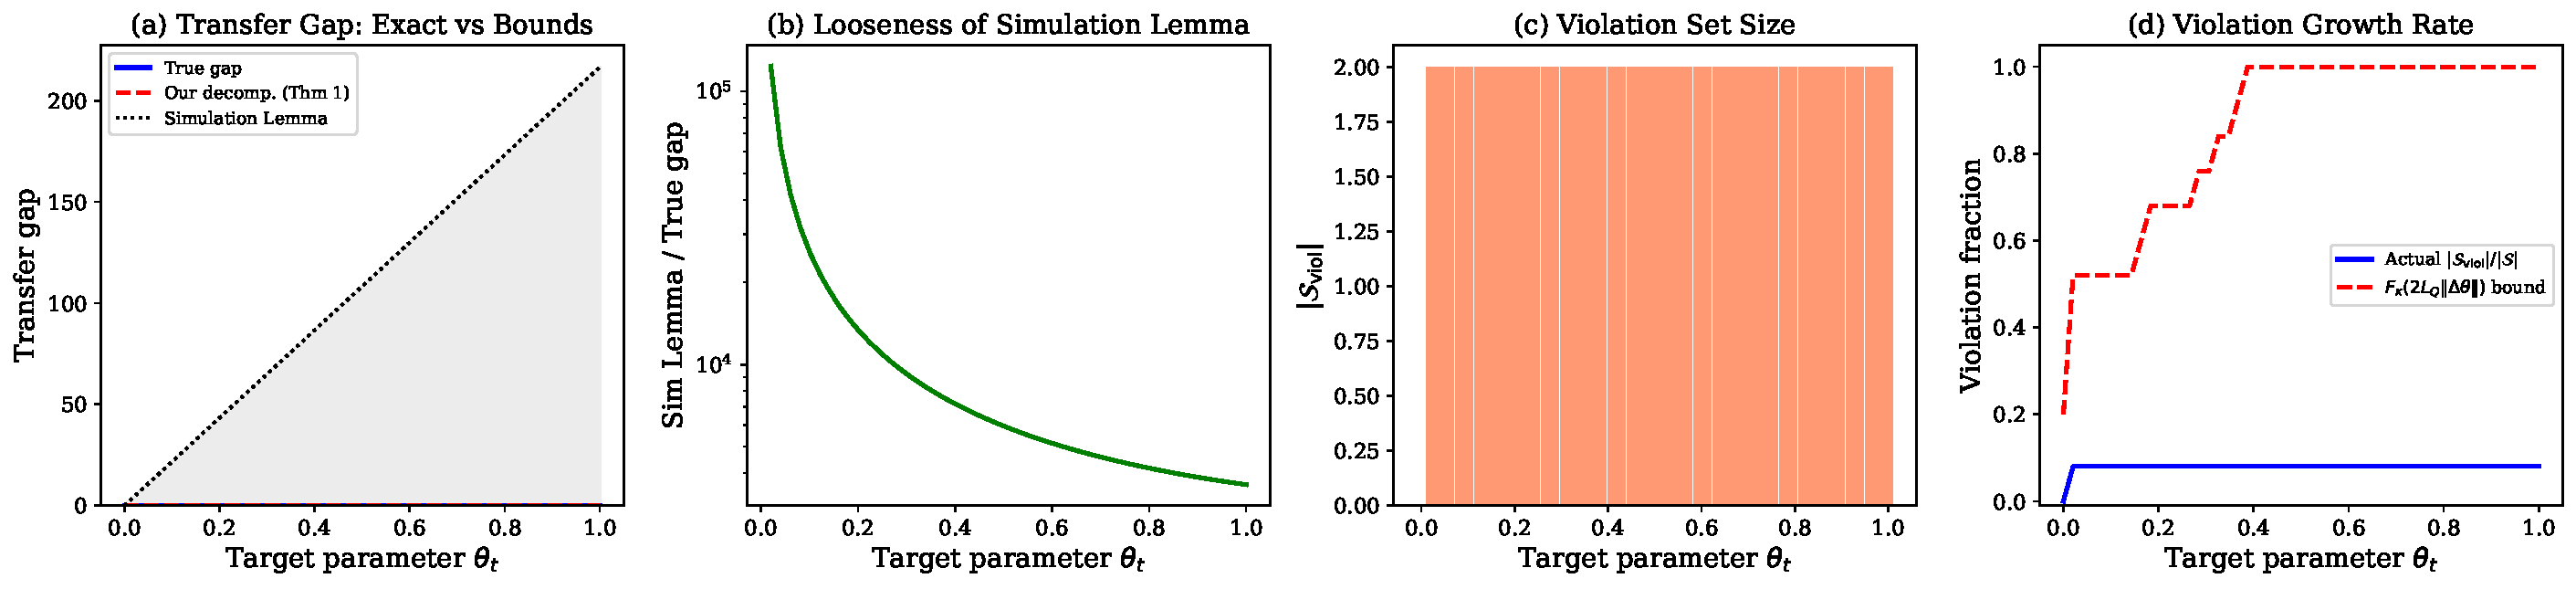
\includegraphics[width=\textwidth]{figures/exp1_transfer_gap.pdf}
\caption{Transfer gap decomposition. (a) Our decomposition (Thm.~\ref{thm:transfer-gap}) matches the true gap; the Simulation Lemma is orders of magnitude loose. (b) Looseness ratio (log scale). (c) $|\Sviol| \leq 2$ out of 25 states. (d) Violation growth: $F_\kappa(2L_Q\|\Delta\theta\|)$ upper-bounds the actual violation fraction (Thm.~\ref{thm:violation-growth}).}
\label{fig:transfer-gap}
\end{figure}

% ────────────────────────────────────────────────────────────
% §7.2 Quadratic Degradation in LQR moved to Appendix~\ref{app:exp-lqr}
% ────────────────────────────────────────────────────────────

% ────────────────────────────────────────────────────────────
\subsection{Comparison with Transfer Baselines}
\label{sec:exp-baselines}
% ────────────────────────────────────────────────────────────

\paragraph{Setup.} $10 \times 10$ grid with two competing goals, wind, and ice ($\theta \in \R^3$). Sources have \emph{heterogeneous reward scales}: each source's Q-values are multiplied by a random factor in $[1/r, r]$ for scale range $r$, simulating environments with different reward magnitudes. We compare: Ordinal (majority-vote, $K=30$), Domain Randomization (solve mean MDP with scaled rewards), Q-Averaging (mean of scaled Q-values), Robust (maximin), and Single Source.

\paragraph{Results.} The ordinal policy is scale-invariant by construction: its transfer gap stays at $4.6$ across all scale ranges $r$ (Figure~\ref{fig:baselines}(c)), while Q-Averaging degrades from $8.2$ to $12.9$ and DR from $4.9$ to $5.8$ as $r$ grows from $1$ to $50\times$. Overall, Ordinal (avg.\ gap $17.4$) beats Q-Averaging ($25.2$), Robust ($39.2$), Single Source ($19.8$) and matches DR ($17.1$); ordinal beats DR in regions far from the source center (Figure~\ref{fig:baselines}(f)).

\begin{figure}[t]
\centering
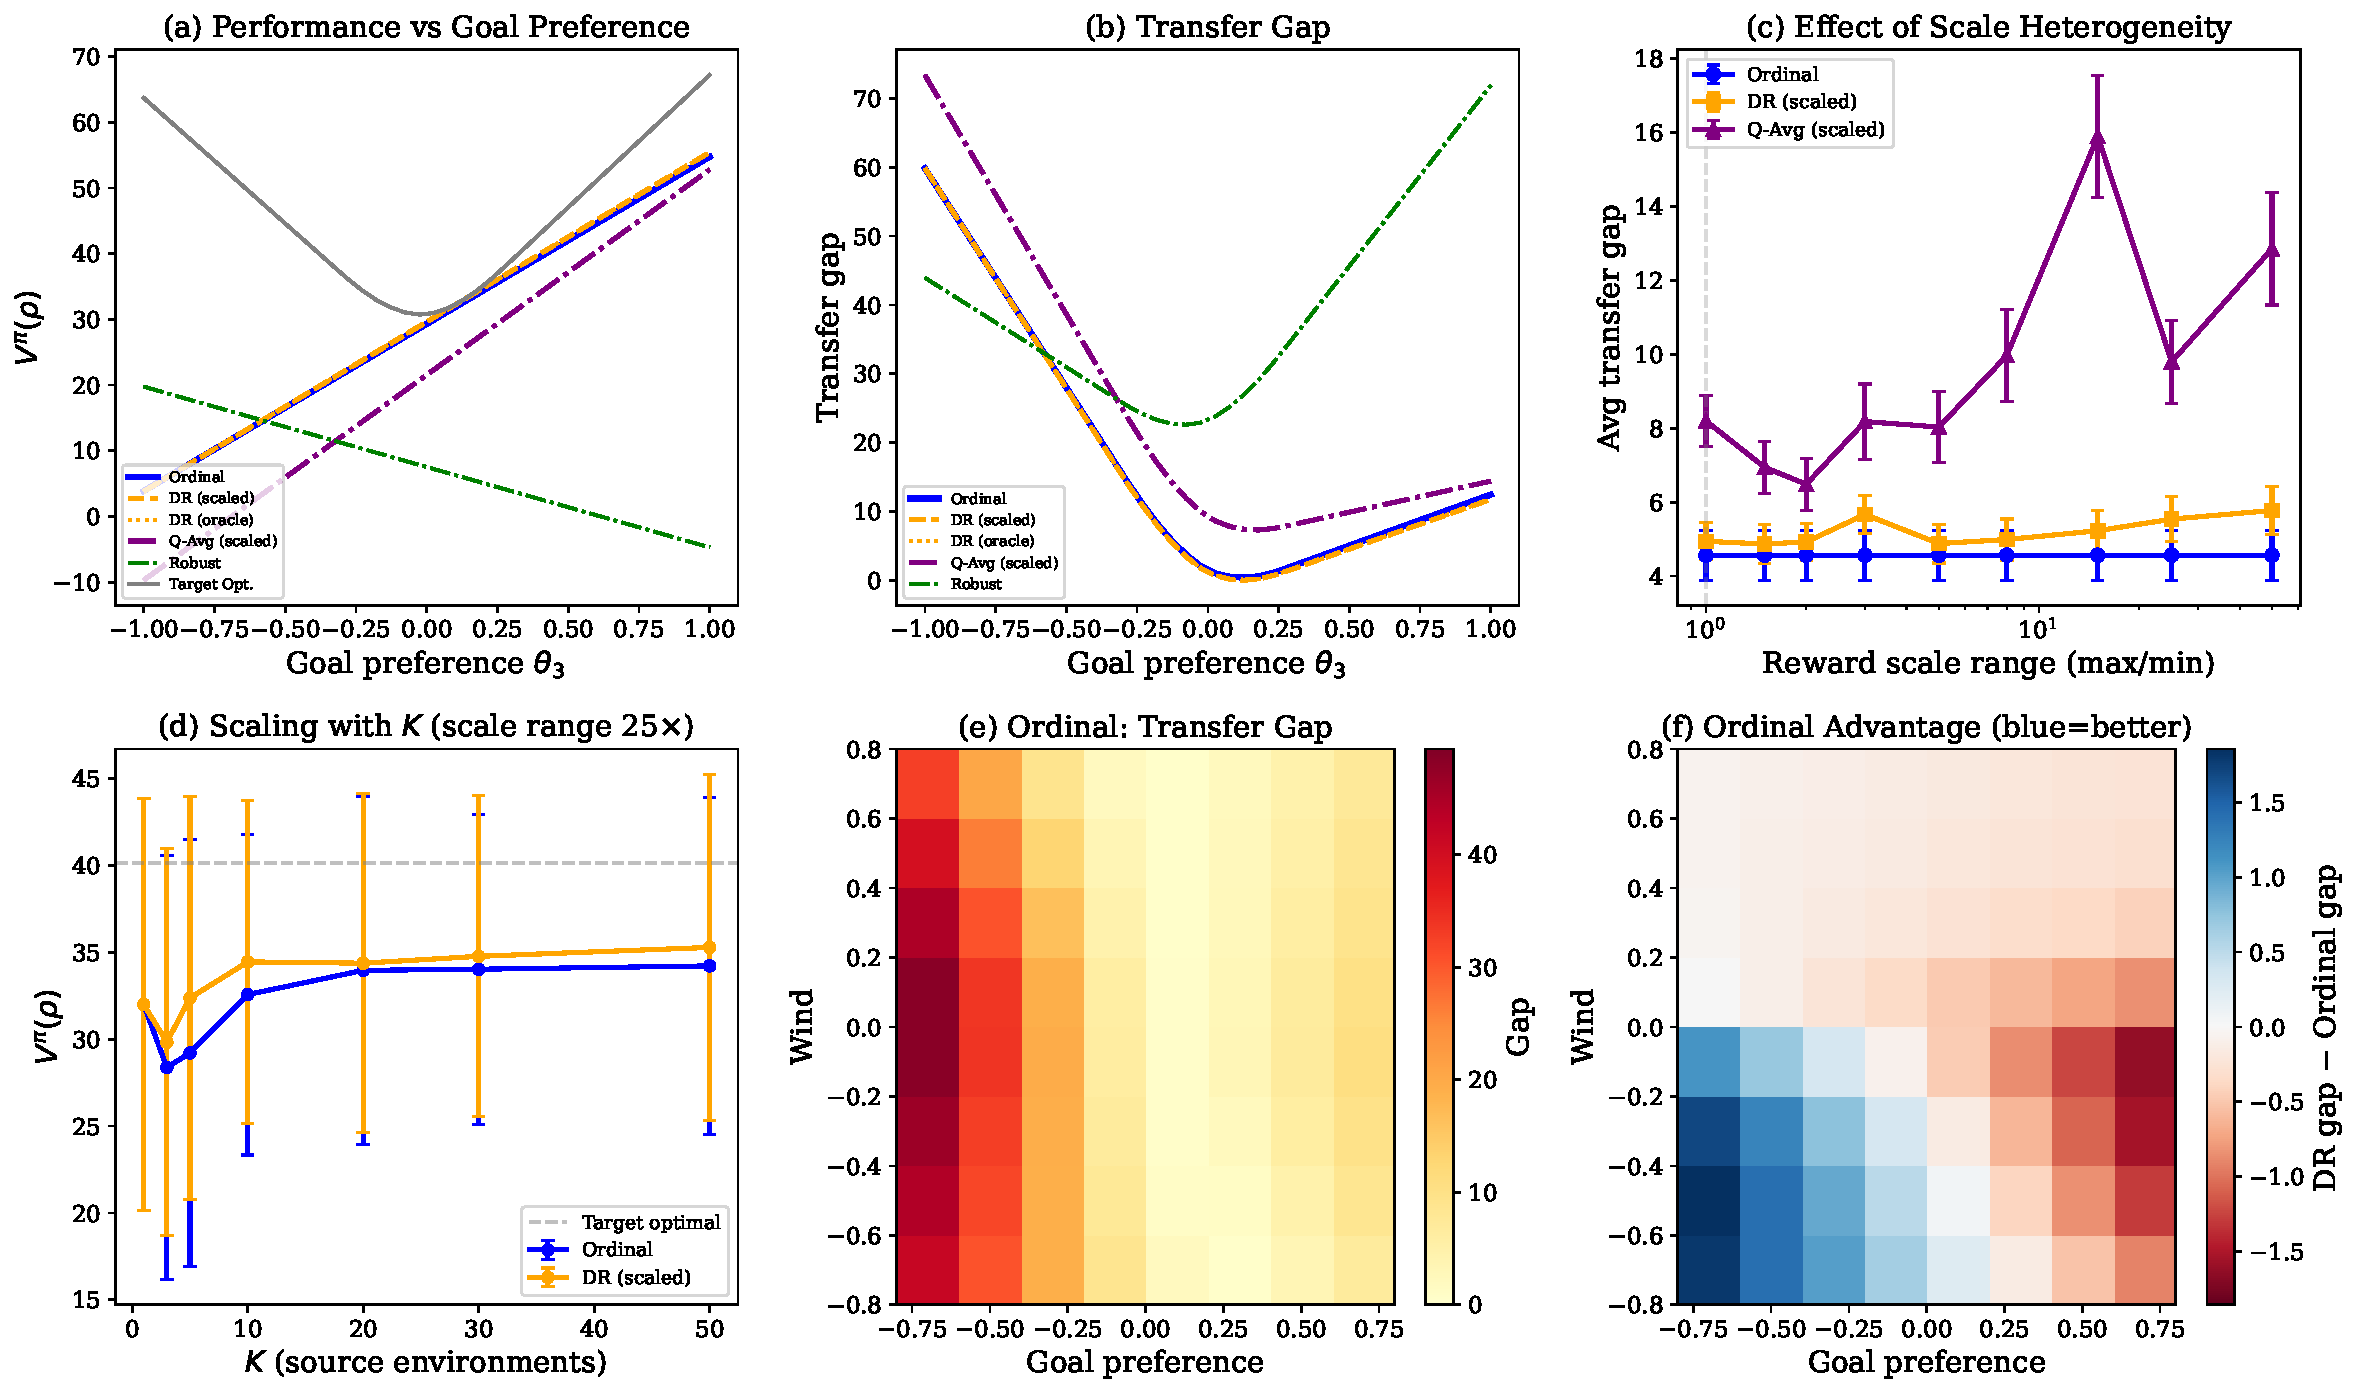
\includegraphics[width=\textwidth]{figures/exp6_baselines.pdf}
\caption{Baseline comparison on $10 \times 10$ grid with heterogeneous reward scales. (a) Performance vs.\ goal preference. (b) Transfer gap. (c) Ordinal gap is flat (scale-invariant) while Q-Averaging and DR degrade with scale heterogeneity. (d) Scaling with $K$. (e) Ordinal gap heatmap. (f) Ordinal advantage over DR (blue = ordinal better).}
\label{fig:baselines}
\end{figure}

% ────────────────────────────────────────────────────────────
\subsection{Neural Policy Transfer: DQN, Gymnasium, and MuJoCo}
\label{sec:exp-neural}
% ────────────────────────────────────────────────────────────

We now test whether ordinal transfer extends to \emph{neural} policies trained from scratch, across three settings of increasing complexity.

\paragraph{Discrete CartPole (DQN).}
\label{sec:exp-dqn}
DQN agents (2-layer MLP, 64 units) on 4-action CartPole (forces $\{-10,-3,+3,+10\}$\,N) at 6 gravities in $[6, 19]$\,m/s$^2$. Directional OC between the source ($g{=}9.8$) and LQR-optimal decays smoothly from $\approx 0.95$ to $\approx 0.75$; majority vote maintains agreement $=1.0$ up to $100\times$ rescaling, while Q-averaging drops to $0.81$ (Figure~\ref{fig:dqn}, Appendix~\ref{app:additional-exp}).

\paragraph{Gymnasium benchmarks (unmodified).}
\label{sec:exp-gymnasium-benchmark}
\texttt{CartPole-v1} (discrete, DQN, 3 seeds, 11 gravities) and \texttt{Pendulum-v1} (continuous, analytical LQR, 20 gravities) rule out custom-environment artifacts. On CartPole-v1, ensemble-averaged OC declines with $|\Delta g|$ and majority vote holds $=1.0$ up to $500\times$ rescaling while Q-averaging degrades (Figure~\ref{fig:gym-bench}, top). On Pendulum-v1, the transfer gap grows with log-log slope $\approx 1.88$ and gain/action displacement are linear in $|\Delta g|$, matching Theorems~\ref{thm:quadratic-subopt}--\ref{thm:action-displacement} (Figure~\ref{fig:gym-bench}, bottom).

\begin{figure}[t]
\centering
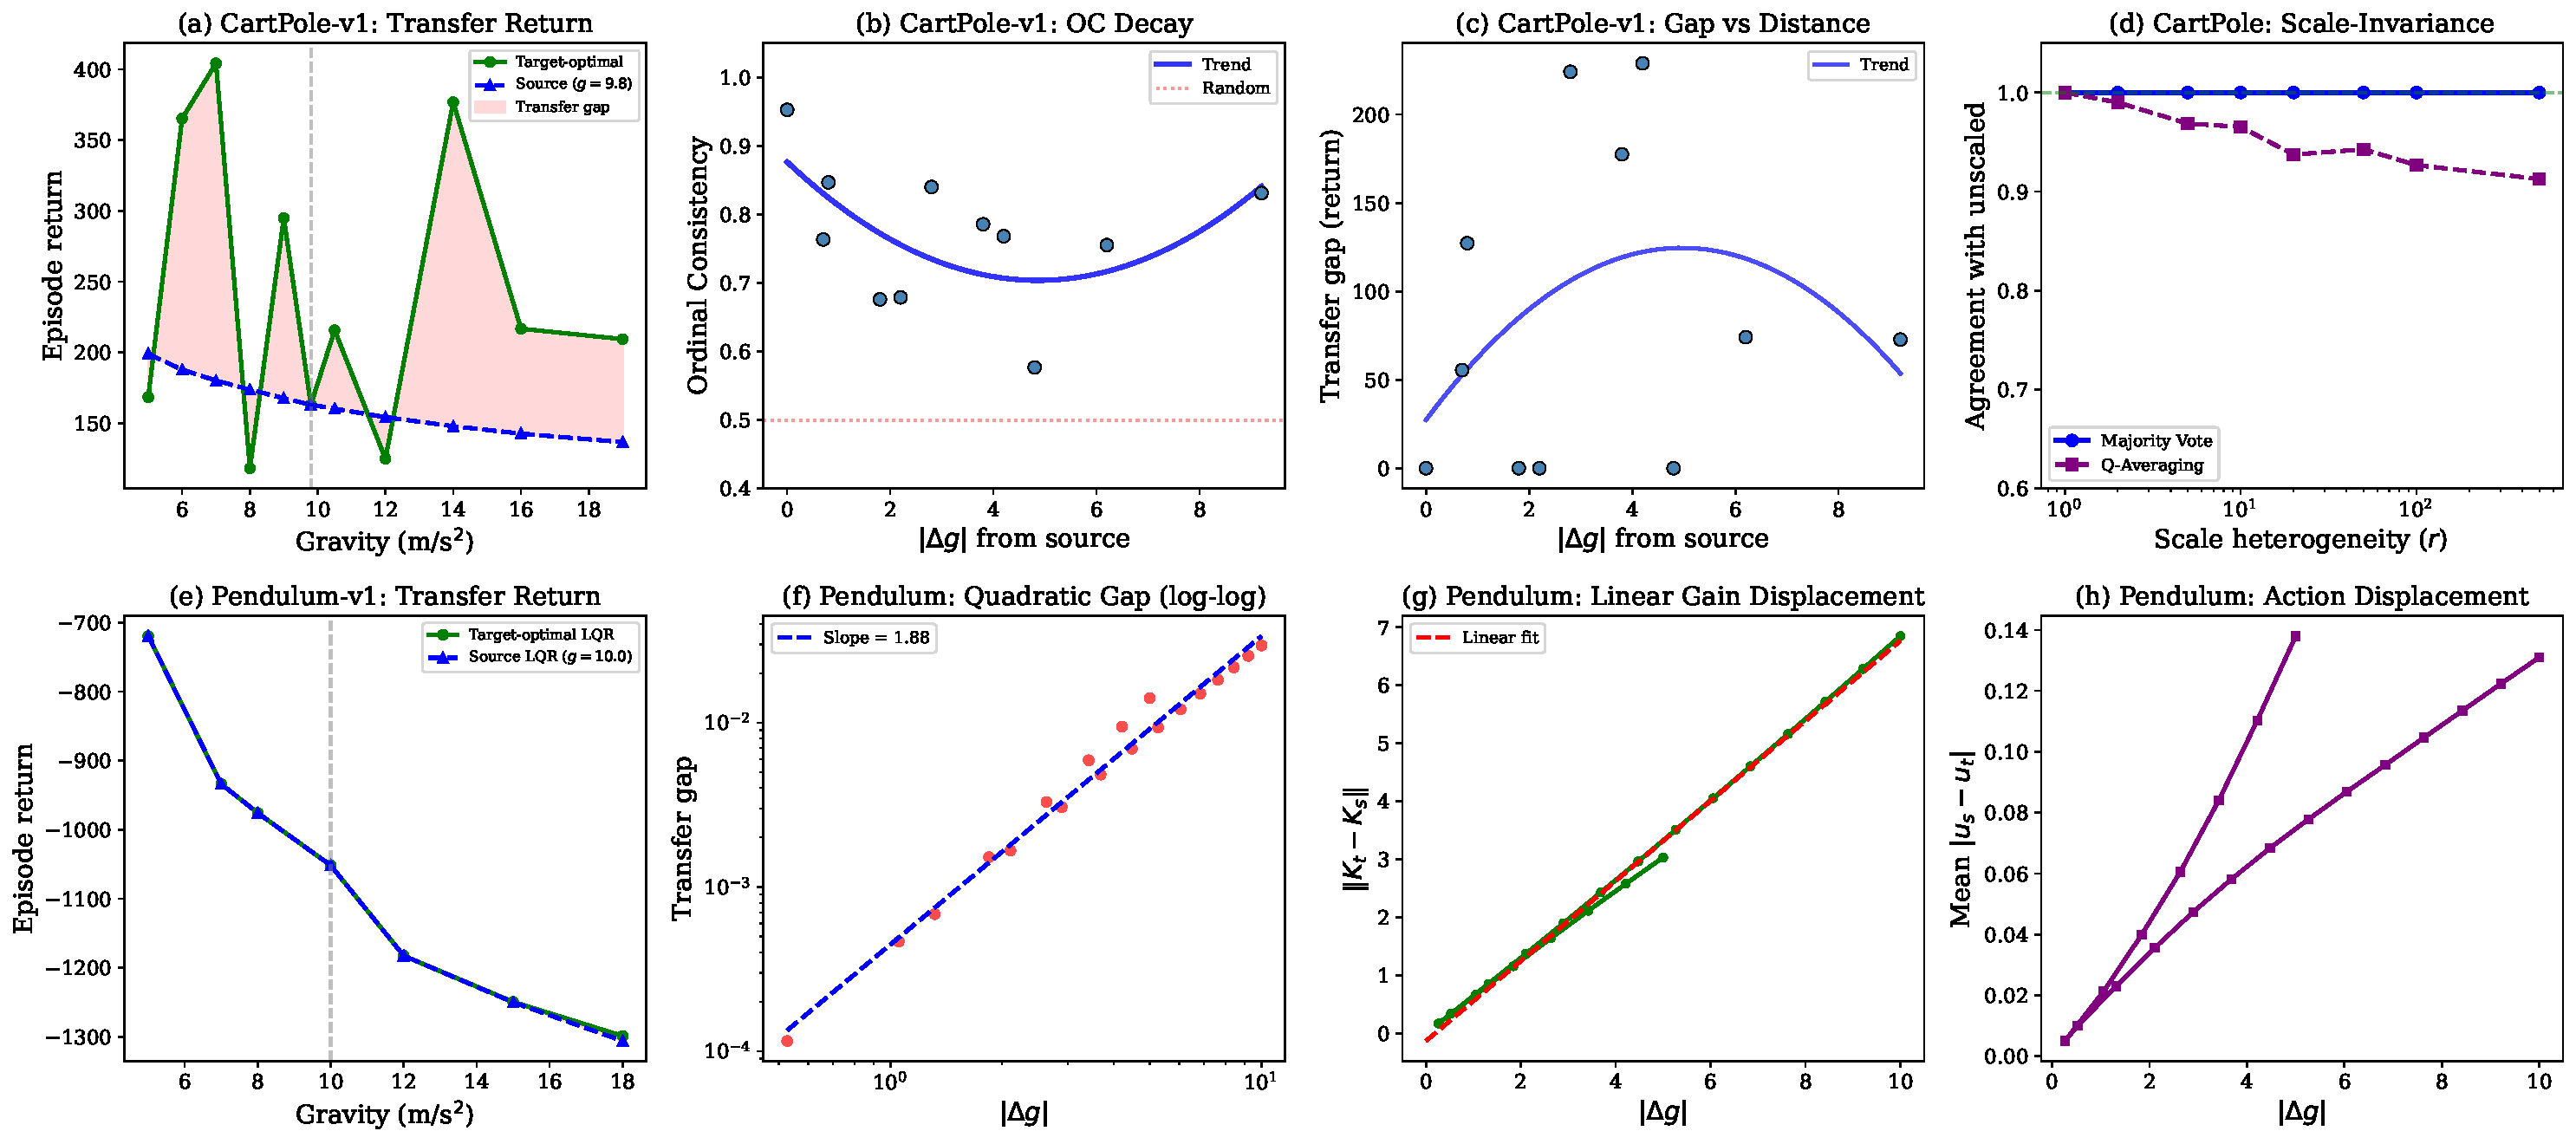
\includegraphics[width=\textwidth]{figures/exp9_gymnasium_benchmark.pdf}
\caption{Gymnasium benchmarks. Top: CartPole-v1 (discrete). (a)~Transfer return. (b)~OC trend. (c)~Gap. (d)~Scale-invariance. Bottom: Pendulum-v1 (continuous). (f)~Quadratic gap ($\approx 1.88$). (g)--(h)~Linear displacement.}
\label{fig:gym-bench}
\end{figure}

\paragraph{MuJoCo continuous control (SAC).}
\label{sec:exp-mujoco-transfer}
SAC (Stable-Baselines3, 500K steps) on HalfCheetah-v4 (17D/6D), Ant-v4 (27D/8D), Hopper-v4 (11D/3D) at $g \in \{5,7,9.81,12,15\}$\,m/s$^2$, plus a domain-randomization (DR) baseline over $[5,15]$. Figure~\ref{fig:mujoco-transfer}: \emph{transfer return} degrades smoothly (Hopper steepest, narrow single-leg region); \emph{directional OC} is highest for Ant ($0.75$--$0.79$, least decay), asymmetric for HalfCheetah, and lowest for Hopper ($0.60$--$0.69$, most decay), matching Theorem~\ref{thm:violation-growth}; \emph{scale-invariance}: MV $=1.000$ uniformly while MA falls to $0.70$--$0.87$. \emph{Transfer-gap scaling} (cross-seed mean over seeds $\{42,123,7\}$, Table~\ref{tab:slope-comparison}) stays strictly below the quadratic upper bound of Theorem~\ref{thm:continuous-bound-main} on Hopper ($\approx 1.17$) and HalfCheetah ($\approx 1.20$), the two environments where Assumption~\ref{asm:local-sc} remains valid across the target gravity range. Ant gives $\approx 2.52$, exceeding the bound; Appendix~\ref{app:hessian-diag} traces this to a directional precondition failure at light gravities, so Ant marks the boundary of the theorem's regime rather than refuting it. DR wins at extreme shifts (it trained there); single-gravity agents stay competitive at moderate shifts.

\paragraph{$F_\kappa$ as a neural diagnostic.} From 500 on-policy states per SAC model, Hopper's median gap ($\tilde{\kappa}=0.015$) is ${\sim}20\times$ smaller than Ant's ($0.363$) or HalfCheetah's ($0.258$), consistent with the coarse OC fragility ordering across environments (Figure~\ref{fig:fkappa-neural}). For quantitative prediction, however, median-only summaries are insufficient: Appendix~\ref{app:fkappa-bound} validates Theorem~\ref{thm:violation-growth} on all 12 (env, target) pairs and shows that, after a single per-environment scale calibration, the full CDF shape $\hat F_\kappa(c^* \cdot |\Delta g|)$ explains the measured violation $2.6\times$--$22\times$ better in MSE than a best-fit median-only predictor (Table~\ref{tab:shape-vs-median}), because the latter collapses to a step.

\paragraph{Multi-seed variance.} Across seeds $\{42,123,7\}$, directional-OC decay is stable (std $\leq 0.15$ per cell) and the qualitative claims reproduce. Transfer-gap magnitudes are noisier per seed: occasional $(\text{seed},g)$ cells where the source incidentally matches the target produce non-positive raw gaps that clip to a floor of $1$ before log fitting, and a single such event can shift a 5-point per-seed slope by several units (per-seed std $2.4$--$3.4$ across envs). We therefore aggregate at the cell level before fitting: the cross-seed mean of cell gaps cancels these zero-gap incidents within a cell and is the only stable summary. The headline Ant slope ($\approx 2.52$) is this cross-seed-mean slope, not the per-seed median ($1.72$, contaminated by the seed-$42$ clipping at $g{=}5$ where source returns collapse to $143\pm72$ vs.\ target $1{,}723\pm404$); reporting the median would mask the directional-precondition failure of Appendix~\ref{app:hessian-diag}. Full tables and per-seed breakdowns: Appendix~\ref{app:multiseed}.

\begin{figure}[t]
\centering
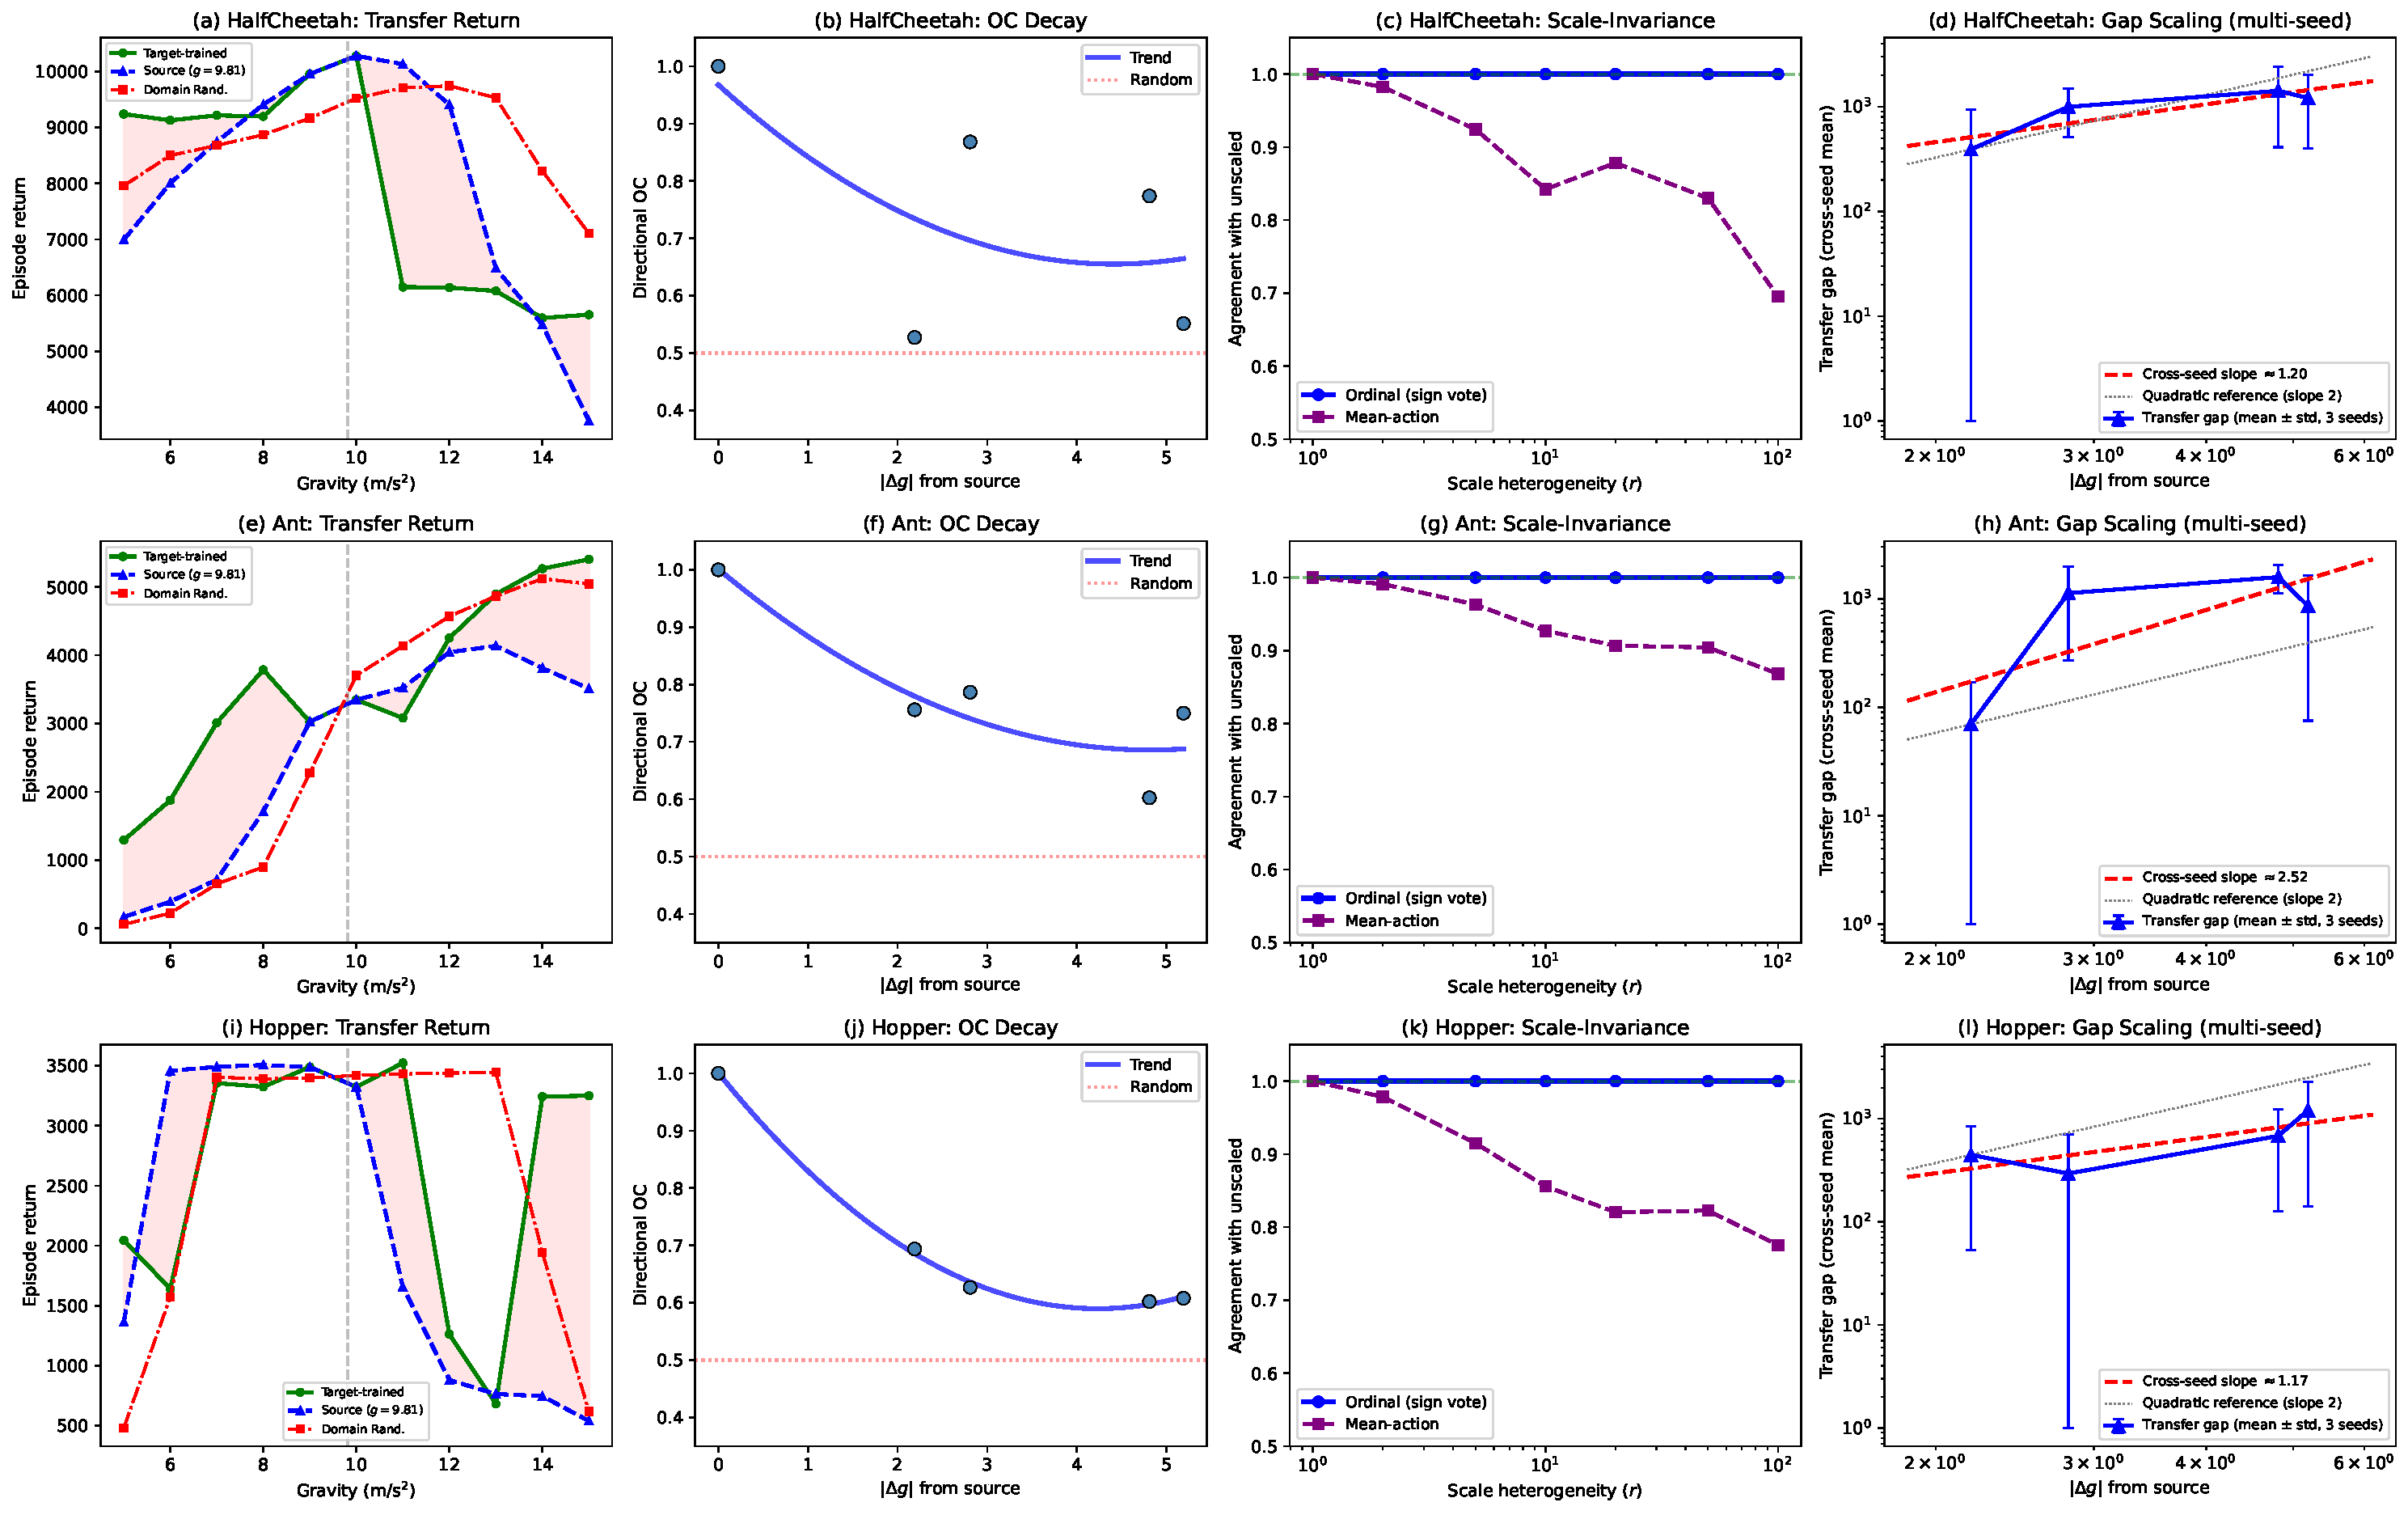
\includegraphics[width=0.68\textwidth]{figures/exp10_mujoco_transfer.pdf}
\caption{MuJoCo SAC (500K). Rows: HalfCheetah, Ant, Hopper. Cols: transfer return at seed $42$ (DR dashed), directional OC at seed $42$, scale-invariance at seed $42$ (MV $=1.000$; MA degrades), and transfer-gap scaling using cross-seed-mean cell-level gaps over seeds $\{42, 123, 7\}$ (error bars $\pm 1$ std). The gap-panel slope labels are the cross-seed fits ($1.20/2.52/1.17$ for HalfCheetah/Ant/Hopper) used as the headline numbers in the body and in Table~\ref{tab:slope-comparison}; the gray dotted line marks the quadratic reference (slope $2$). Under this summary, HalfCheetah and Hopper remain below the quadratic upper bound of Thm.~\ref{thm:continuous-bound-main}, while Ant exceeds it; Appendix~\ref{app:hessian-diag} traces the Ant deviation to a directional precondition failure at light gravities. Seed-$42$ single-fit slopes ($4.56/4.19/1.88$) are reported alongside the Hessian diagnostic in Appendix~\ref{app:hessian-diag} for the regime where the local quadratic model collapses.}
\label{fig:mujoco-transfer}
\end{figure}

\paragraph{Multi-dimensional parameter transfer.} Appendix~\ref{app:exp-multidim} extends the above to $d{=}3$ simultaneous shifts (gravity $\times$ friction $\times$ mass) on HalfCheetah-v4: the source policy stays competitive across all shift magnitudes, and OC decay, scale-invariance, and action displacement depend only on $\|\Delta\thetavec\|$ regardless of which physics parameters vary.

\paragraph{Source-only deploy-or-adapt decision.} A diagnostic is useful only if it improves decisions. For each target gravity $g \neq g_\mathrm{src}$ we decide at source time whether to deploy the source policy zero-shot or fall back to a domain-randomized policy trained on $g\in[5,15]$, scoring the decision by the resulting return. The rule adapts iff $\hat F_\kappa(c\,|\Delta g|) > \tau$ with env-agnostic $c=0.1, \tau=0.5$ (no per-env tuning); $\hat F_\kappa$ is the same source-side CDF used everywhere else. Inline summary (mean return over four non-source gravities, $\hat F_\kappa$ rule vs.\ \emph{always-deploy} / \emph{always-adapt} (DR) / oracle): \textbf{HalfCheetah} $\mathbf{8{,}194}$ vs.\ $7{,}143/8{,}396/8{,}396$; \textbf{Ant} $\mathbf{2{,}509}$ vs.\ $2{,}197/2{,}561/2{,}642$; \textbf{Hopper} $\mathbf{1{,}988}$ vs.\ $1{,}555/1{,}988/2{,}266$. The rule attains $75\%$ decision accuracy vs.\ oracle in all three envs, captures ${>}94\%$ of the oracle return, and strictly beats \emph{always-deploy} everywhere; unlike \emph{always-adapt} it correctly flags Ant $g{=}7$ (where the source policy is the better deployment) from source data alone. Per-cell breakdown and the full table: Appendix~\ref{app:deploy-or-adapt}.
